\documentclass{article}
\usepackage[a4paper,left=2.5cm,right=2.5cm,top=2.5cm,bottom=2.5cm]{geometry}
\usepackage[bahasa]{babel}
\usepackage{graphicx}
\graphicspath{{./images/}}

% \usepackage{lipsum}
% \usepackage{graphicx}
% \usepackage{hyperref}
\begin{document}
\begin{center}
    \textbf{UJIAN Manajemen Pemasaran Bisnis Digital}\\
    62/MMSI/SIB 91122010 Ilman Samhabib
\end{center}
\section*{Soal 1}
Setiap kata \textbf{marketing} 
dibawah ini bisa didefinisikan sama yaitu proses 
memenuhi kebutuhan 
dan keinginan manusia melalui pertukaran 
produk ataupun menyediakan layanan, 
dengan menggunakan strategi tertentu 
seperti dengan promosi produk/layanan, 
menentukan harga, 
juga distribusi yang efisien. 
Strategi-strategi ini bertujuan mendapatkan 
lebih banyak pelanggan 
juga meningkatkan tingkat familiaritas pelanggan terhadap 
hal yang dipromosikan
agar terjalin tingkat kesetiaan  
/ \emph{costumer retention} tertentu dengan pelanggan yang ada 
ataupun 
calon pelanggan potensial\\
Jadi pada dasarnya meningkatkan/memberi 
\emph{value} bagi pelanggan dengan harapan 
mendapatkan \emph{value} lebih 
dari pelanggan itu juga(Kotler \& Amstrong).
\\

\noindent Setiap istilah dibawah ini akan menggunakan 
platform dan strategi 
\emph{marketing} berbeda, 
tetapi seringkali penggunaan istilah ini merujuk pada 
hal yang sama dengan istilah lainnya.\\

\noindent\textbf{Digital Marketing} dan \textbf{cyber marketing} merupakan 
marketing dengan memanfaatkan 
\textbf{channel digital} yang dapat lebih efisien dan terukur
dalam menyampaikan promosi 
dan menentukan sentimen pelanggan dibandingkan dengan 
menggunakan media tradisional dalam kegiatan \emph{marketing}\\

\noindent\textbf{Online Marketing}, 
\textbf{Internet Marketing}, 
adalah \textbf{channel digital} 
dalam \emph{marketing} yang memanfaat peralatan yang sudah 
terkoneksi secara luas dalam jaringan internet.\\

\noindent Begitupun dengan \textbf{Electronic Marketing} tetapi kerap kali ini lebih menjurus 
pada taktik penggunaan kanal yang lebih personal, 
seperti pesan email dan semacamnya,

\noindent\textbf{Web based Marketing} adalah \textbf{channel digital} 
dalam \emph{marketing} yang memanfaatkan sebuah \emph{web site}\\

\noindent Sedangkan \textbf{Mobile Marketing} adalah proses \emph{marketing} dengan memanfaatkan \emph{handphone} ataupun perangkat praktis dan  \emph{mobile} yang tentunya memiliki taktik dan alat-alat pengukur berbeda.\\

\noindent Begitupun \textbf{Social Media Marketing} adalah proses \emph{marketing} dengan memanfaatkan \emph{social media} yang dapat diakses dengan \emph{handphone} ataupun perangkat lain yang terhubung internet, tetapi menggunakan taktik berbeda, seperti taktik marketing menggunakan \emph{influencer}\\


\section*{Soal 2}
Produk yang ditawarkan: Aksesoris dan komponen 
desktop-komputer (PC) laptop. \\
Layanan yang ditawarkan: Perakitan PC dengan komponen yang dapat dipilih.
Sasaran website adalah para pelanggan yang mencari berbagai macam aksesoris komputer
\smallbreak\noindent
\begin{minipage}{0.30\textwidth}
    Web berisi banner besar yang berisi promosi-promosi ataupun barang barang yang featured ataupun yang mendapatkan diskon,
    disini website berusaha memenuhi \textbf{fungsi promosi}
\end{minipage}
\hspace*{0.04\textwidth}
\begin{minipage}{0.65\textwidth}
    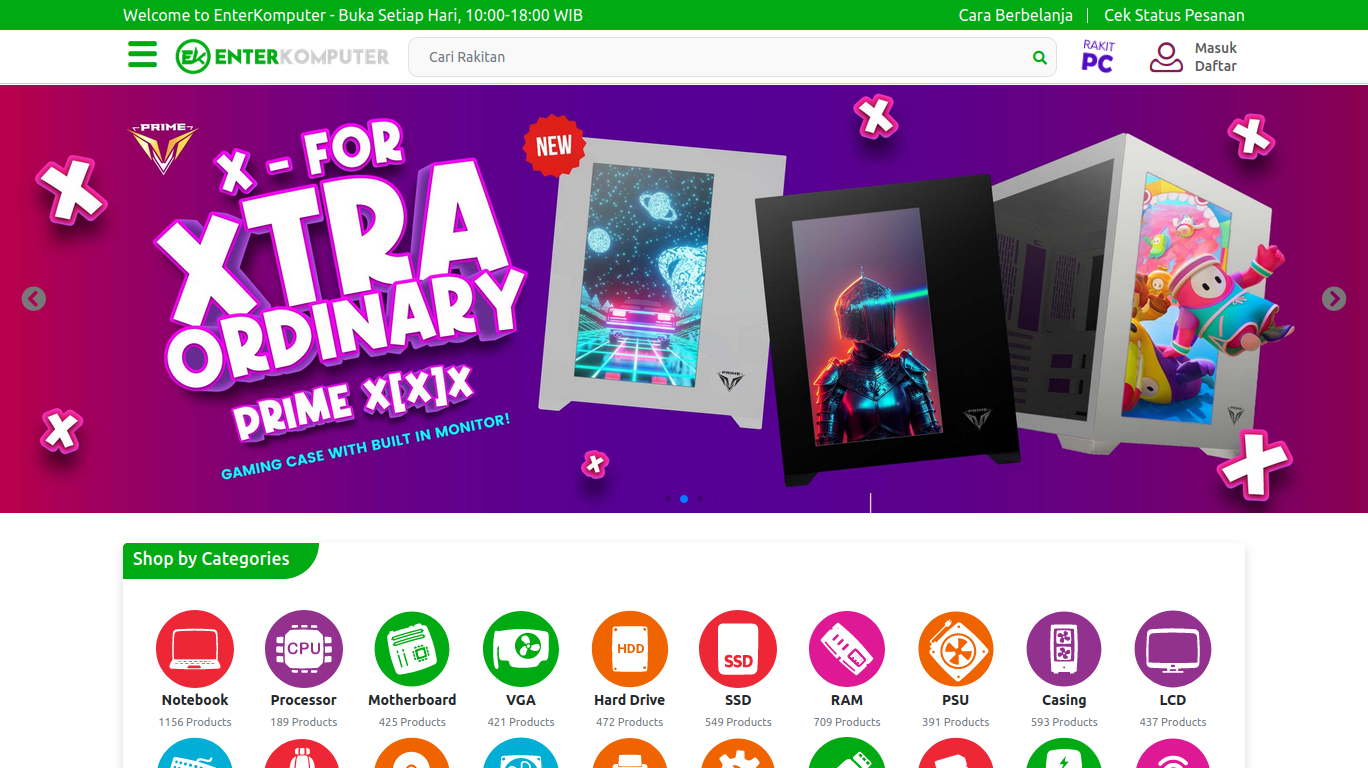
\includegraphics[width=\textwidth]{file-34.png}
\end{minipage}
\\
\begin{minipage}{0.30\textwidth}
    lalu diikuti dengan katalog barang yang dijual
\end{minipage}
\hspace*{0.04\textwidth}
\begin{minipage}{0.65\textwidth}
    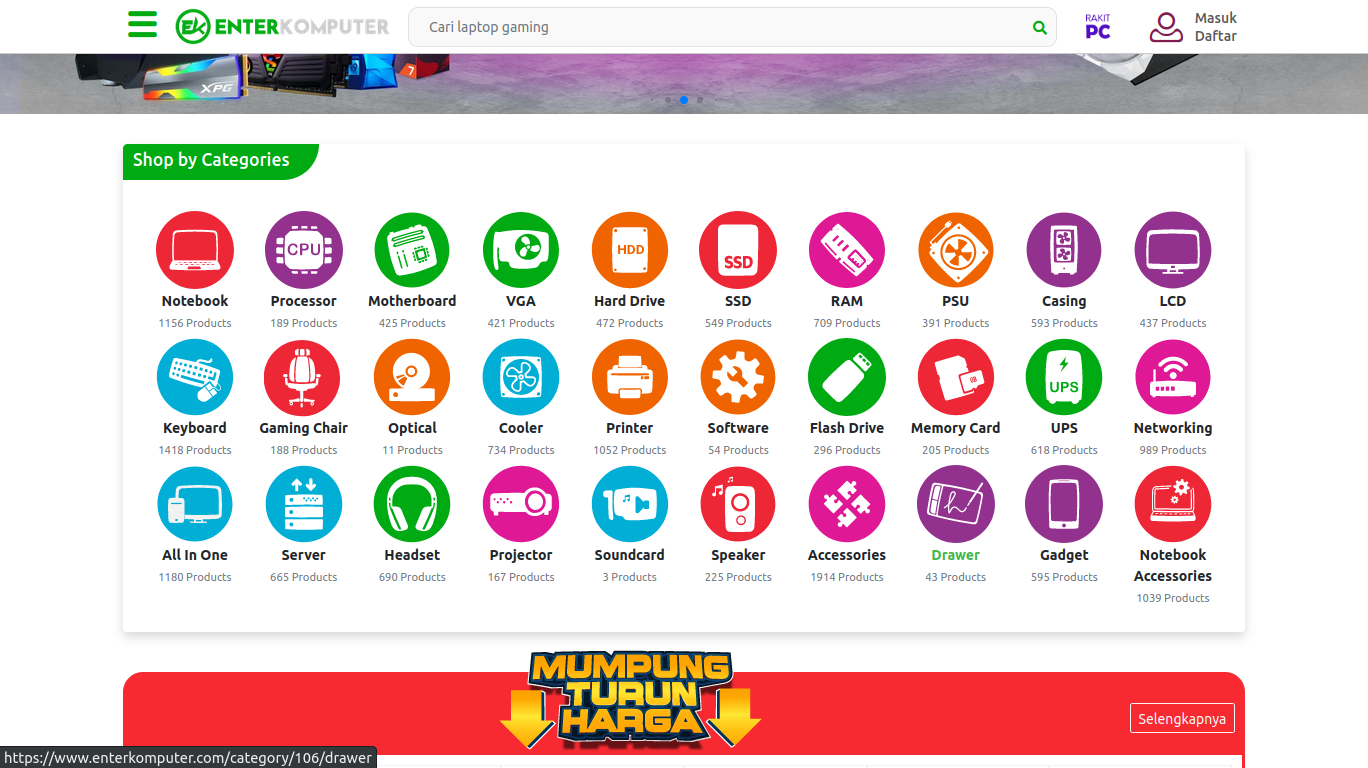
\includegraphics[width=\textwidth]{file-33.png}
\end{minipage}
\\
\begin{minipage}{0.30\textwidth}
    ini adalah bagian event, dan menampilkan katalog barang yang terkena diskon karena event teretentu, \textbf{fungsi promosi}
\end{minipage}
\hspace*{0.04\textwidth}
\begin{minipage}{0.65\textwidth}
    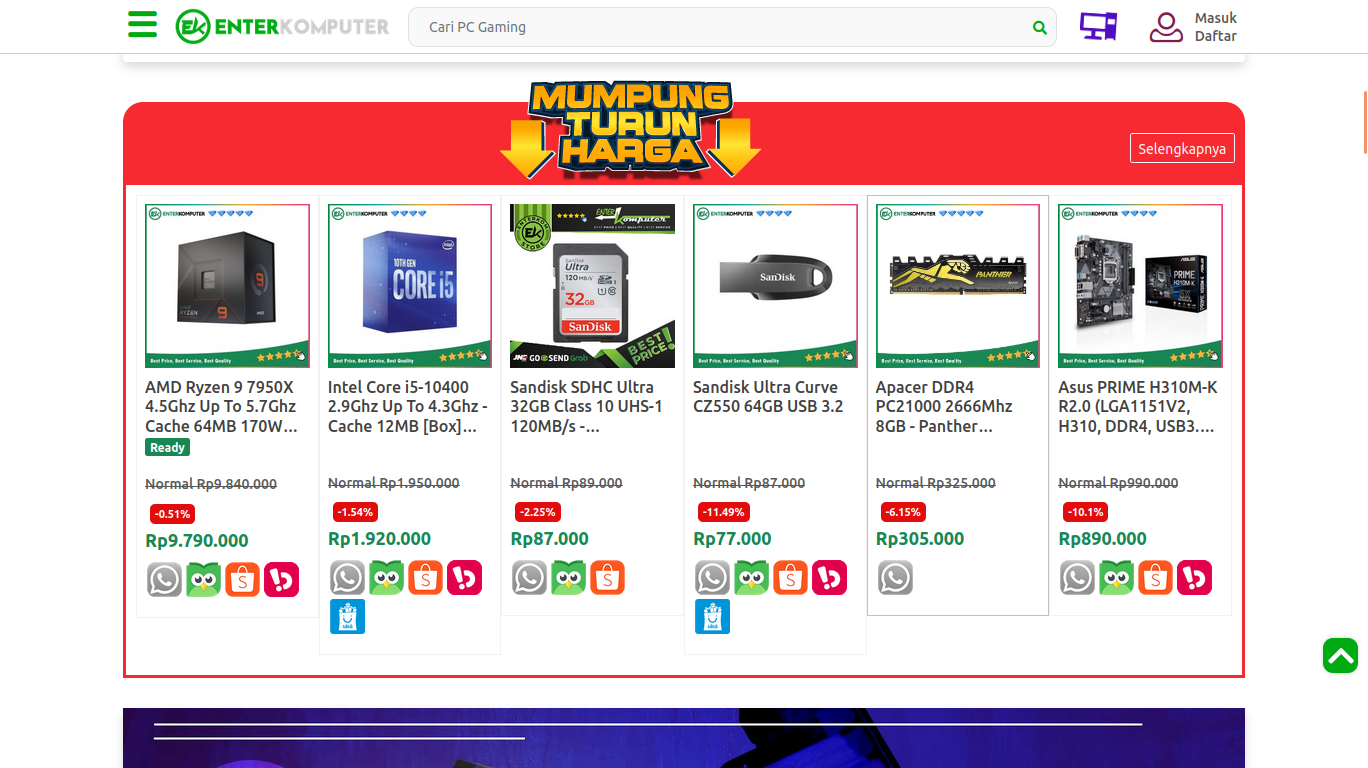
\includegraphics[width=\textwidth]{file-32.png}
\end{minipage}
\\
\begin{minipage}{0.30\textwidth}
    masih dihalaman depan, pada seksi ini dapat diakses layanan perakitan komputer, \textbf{fungsi penyelarasan} dan \textbf{fungsi promosi}
\end{minipage}
\hspace*{0.04\textwidth}
\begin{minipage}{0.65\textwidth}
    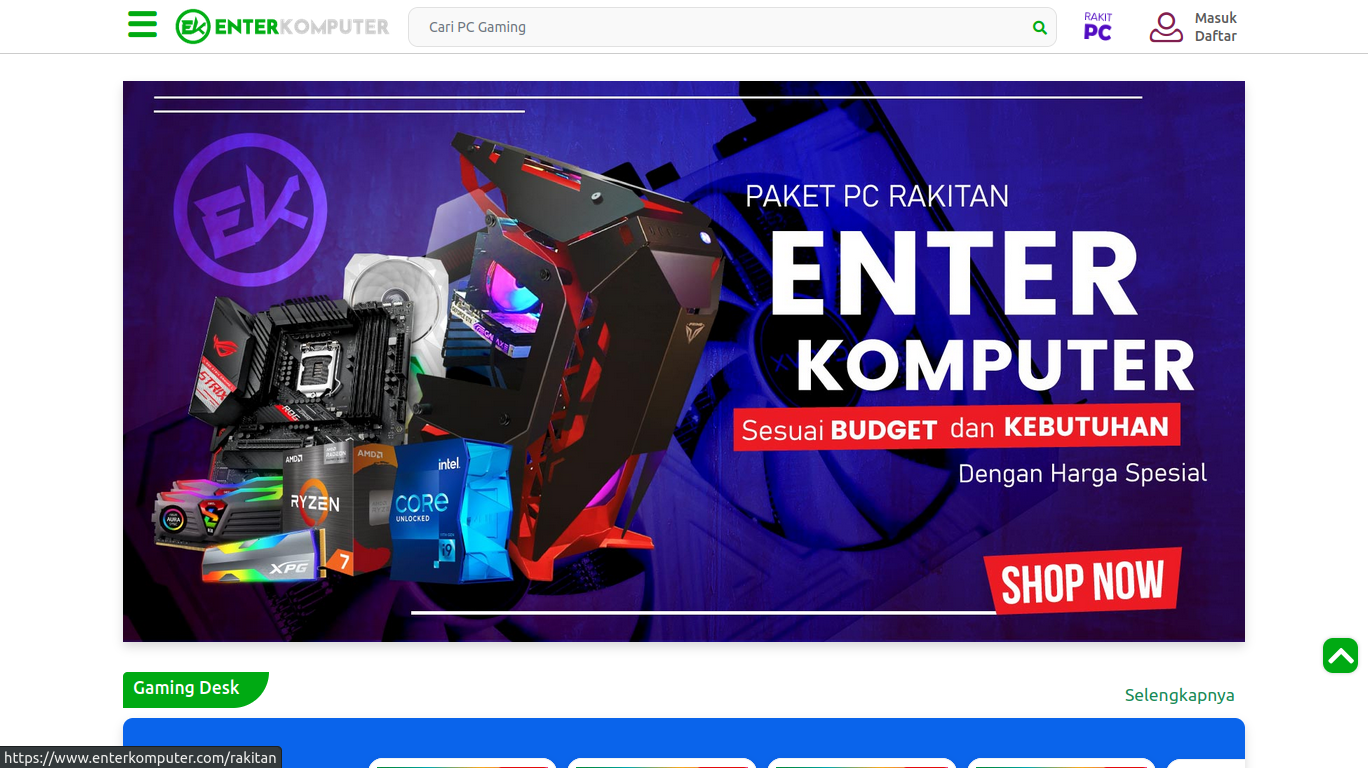
\includegraphics[width=\textwidth]{file-31.png}
\end{minipage}
\\
\begin{minipage}{0.30\textwidth}
    masih dihalaman depan, ditawarkan juga barang yang terkait dengan barang yang mungkin sering dicari, \textbf{fungsi promosi}
\end{minipage}
\hspace*{0.04\textwidth}
\begin{minipage}{0.65\textwidth}
    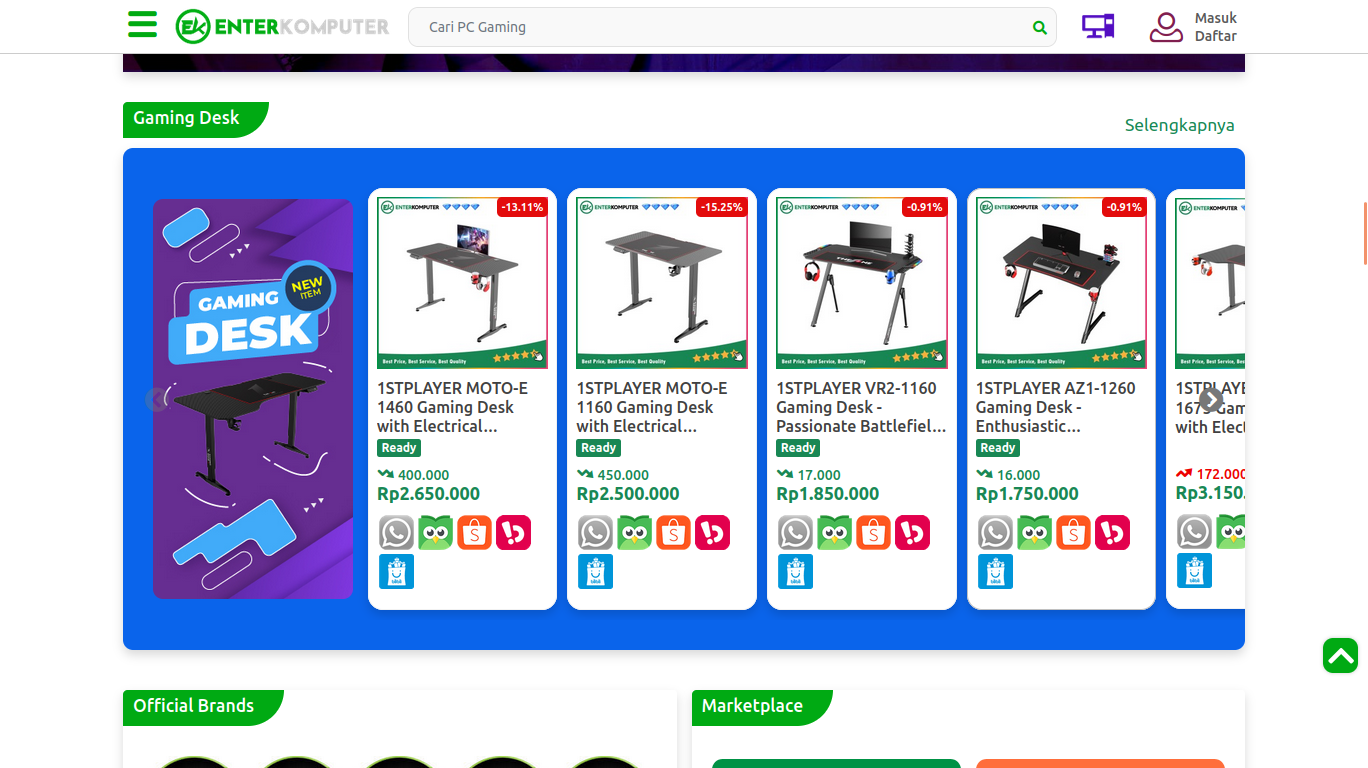
\includegraphics[width=\textwidth]{file-30.png}
\end{minipage}
\\
\begin{minipage}{0.30\textwidth}
    begitupun menampilkan produk yang terkait di bagian ini
\end{minipage}
\hspace*{0.04\textwidth}
\begin{minipage}{0.65\textwidth}
    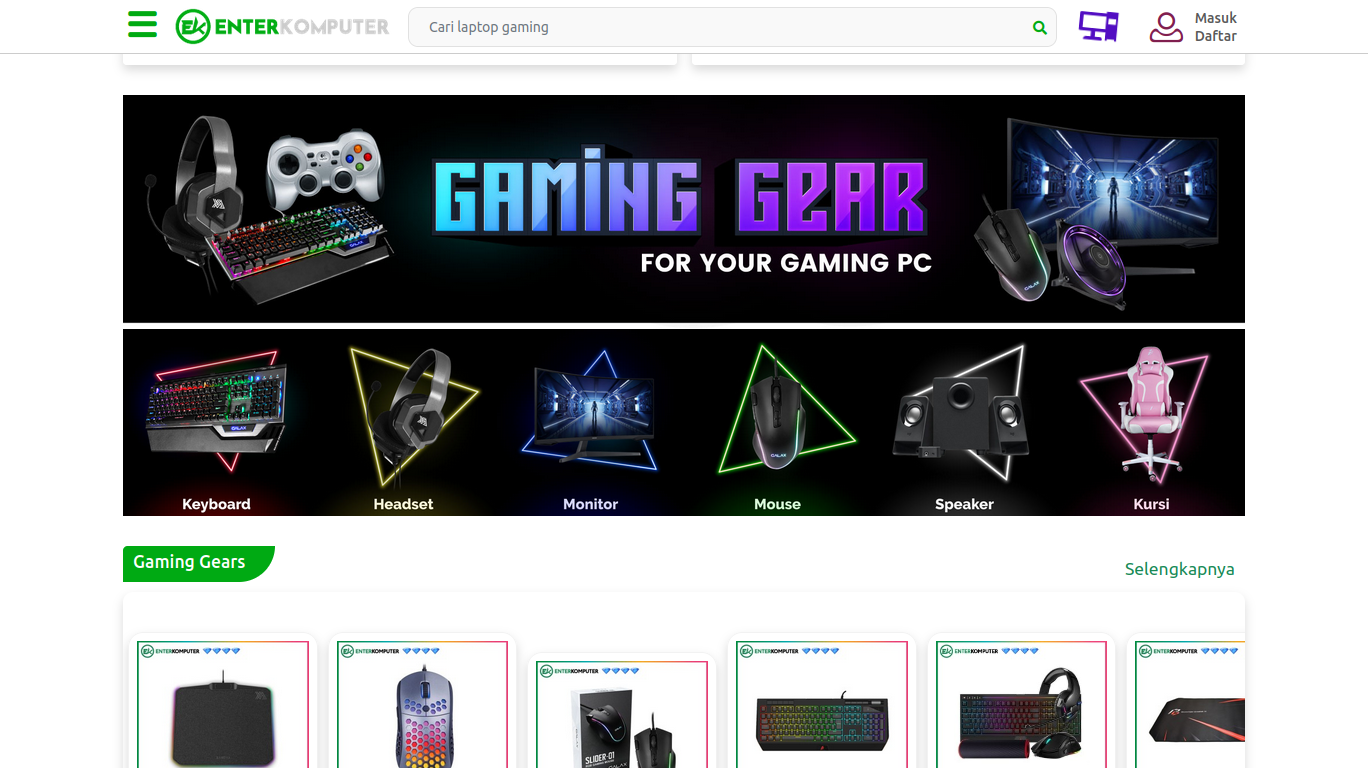
\includegraphics[width=\textwidth]{file-28.png}
\end{minipage}
\\
\begin{minipage}{0.30\textwidth}
    jika user ingin menggunakan platform belanja yang lebih
     terkenal disediakan pula link ke marketplace populer di indonesia, \textbf{distribusi fisik} dan atau \textbf{pembiayaan}
\end{minipage}
\hspace*{0.04\textwidth}
\begin{minipage}{0.65\textwidth}
    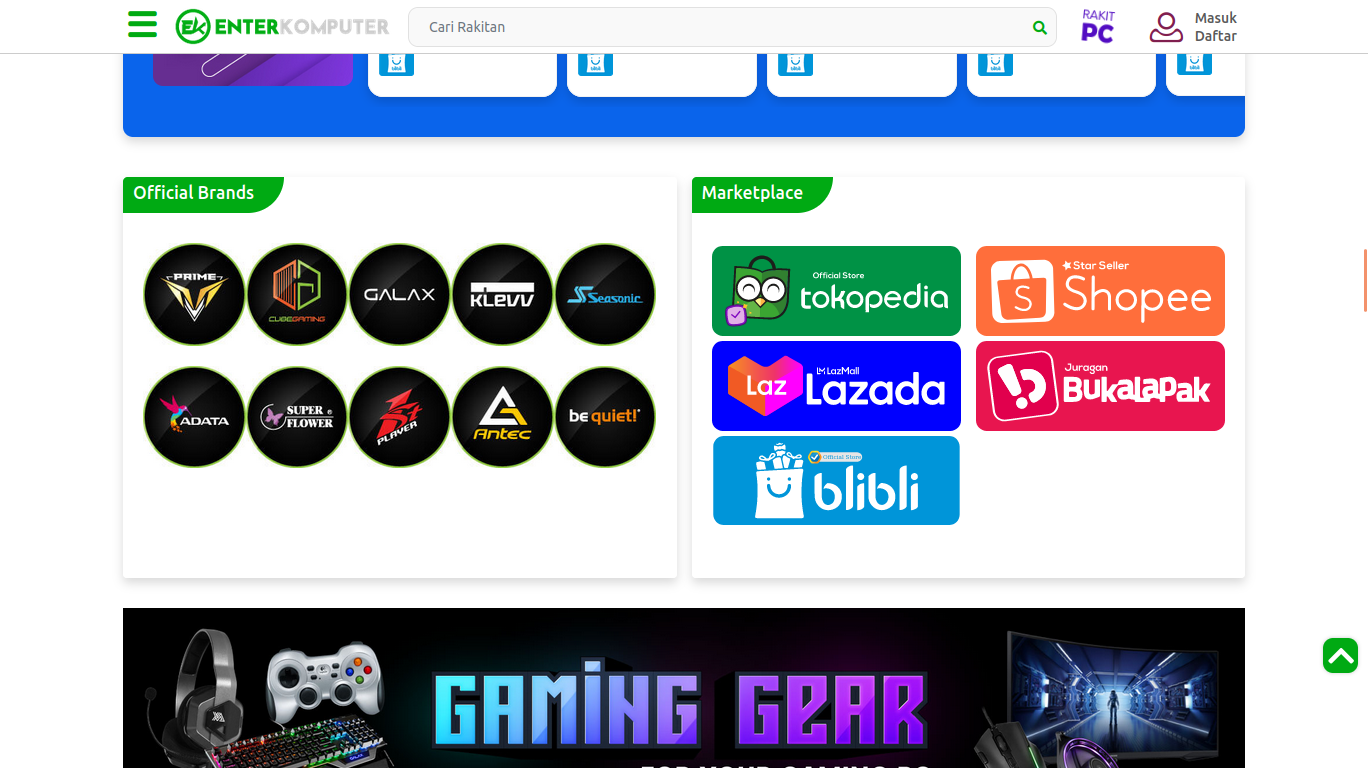
\includegraphics[width=\textwidth]{file-29.png}
\end{minipage}
\\
\begin{minipage}{0.30\textwidth}
    di sini ditampilkan berita terkini yang terkait dengan perakitan 
    dan komponen PC/Laptop, \textbf{fungsi research}
\end{minipage}
\hspace*{0.04\textwidth}
\begin{minipage}{0.65\textwidth}
    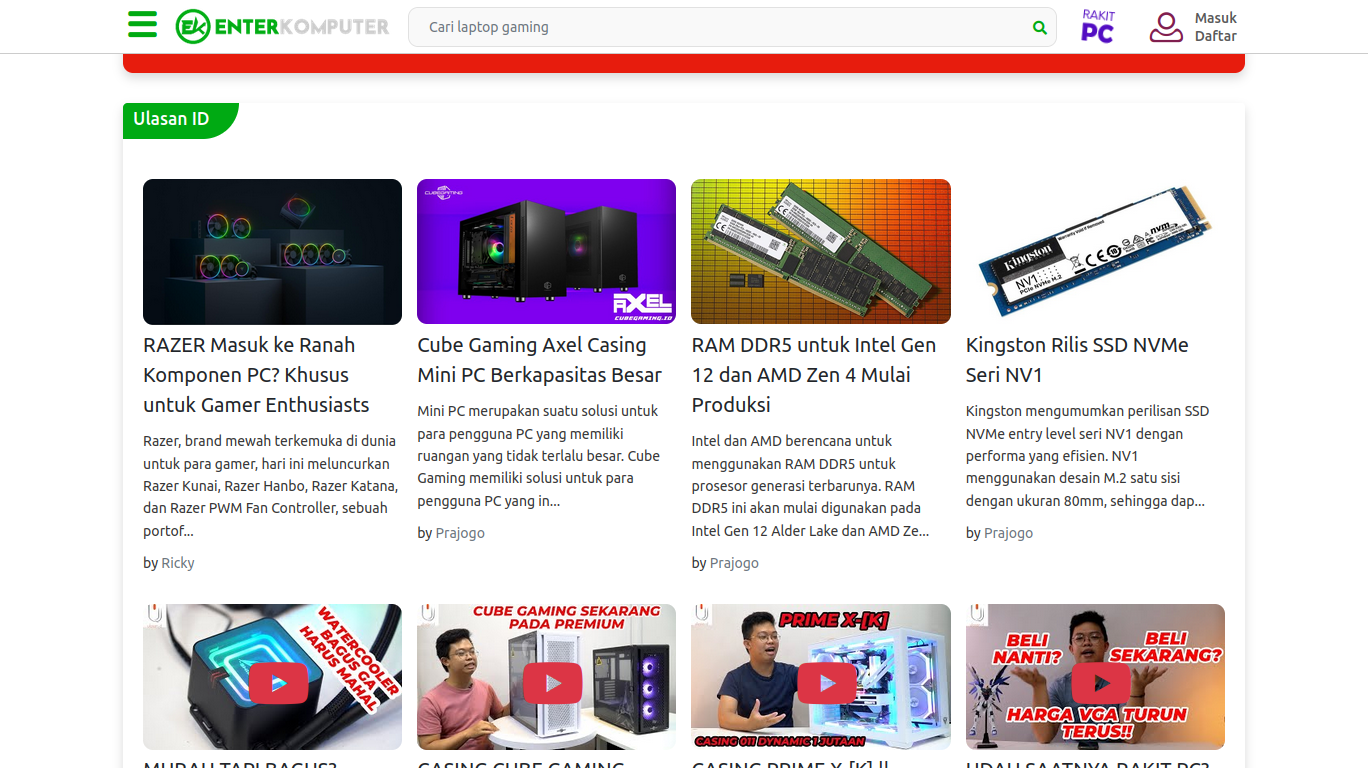
\includegraphics[width=\textwidth]{file-24.png}
\end{minipage}
\\
\begin{minipage}{0.30\textwidth}
    dengan menggunakan analitik yang terkait dengan perilaku browsing pengguna, 
    situs ini dapat merekomendasikan produk tertentu yang mungkin akan dibeli, \textbf{fungsi promosi}
\end{minipage}
\hspace*{0.04\textwidth}
\begin{minipage}{0.65\textwidth}
    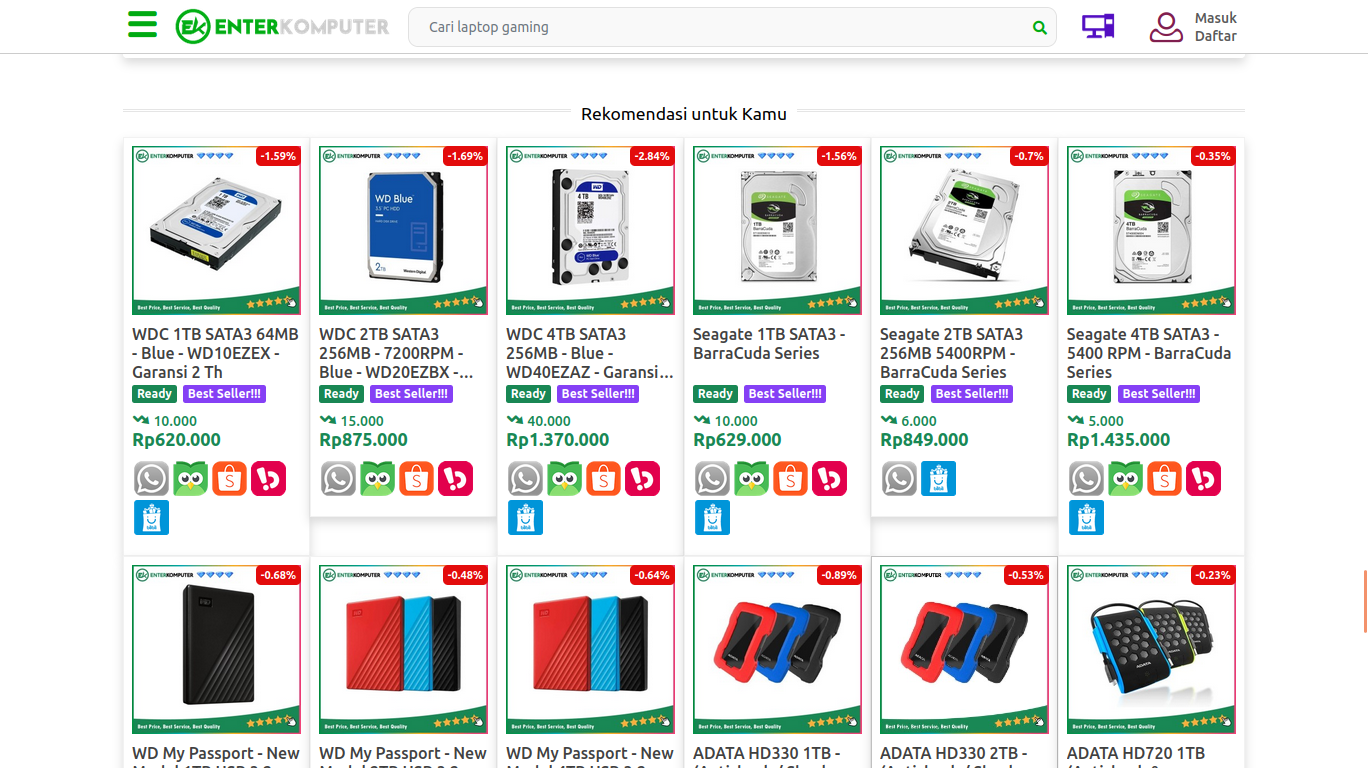
\includegraphics[width=\textwidth]{file-23.png}
\end{minipage}
\\
\begin{minipage}{0.30\textwidth}
    pada bagian bawah dapat dilihat berbagai macam informasi, seperti cara pembayaran dan  jadwal buka toko fisik, dan nomor-nomor yang dapat dihubungi termasuk didalamnya nomor aduan, 
    \textbf{fungsi kontak} dengan pelanggan
\end{minipage}
\hspace*{0.04\textwidth}
\begin{minipage}{0.65\textwidth}
    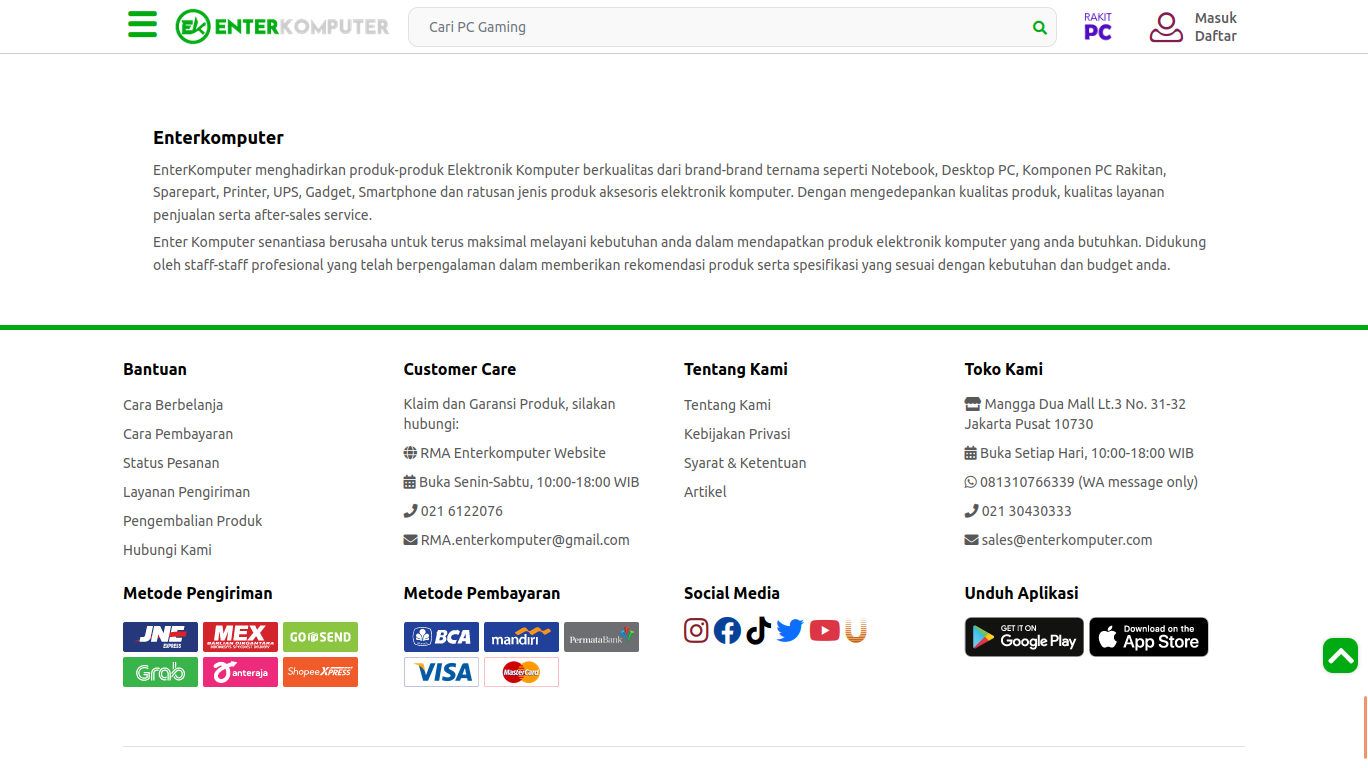
\includegraphics[width=\textwidth]{file-22.png}
\end{minipage}
\\
\begin{minipage}{0.30\textwidth}
    pada bagian bawah dapat dilihat berbagai macam informasi, seperti cara pembayaran dan  jadwal buka toko fisik, dan nomor-nomor yang dapat dihubungi termasuk didalamnya nomor aduan, 
    \textbf{fungsi kontak} dengan pelanggan
\end{minipage}
\hspace*{0.04\textwidth}
\begin{minipage}{0.65\textwidth}
    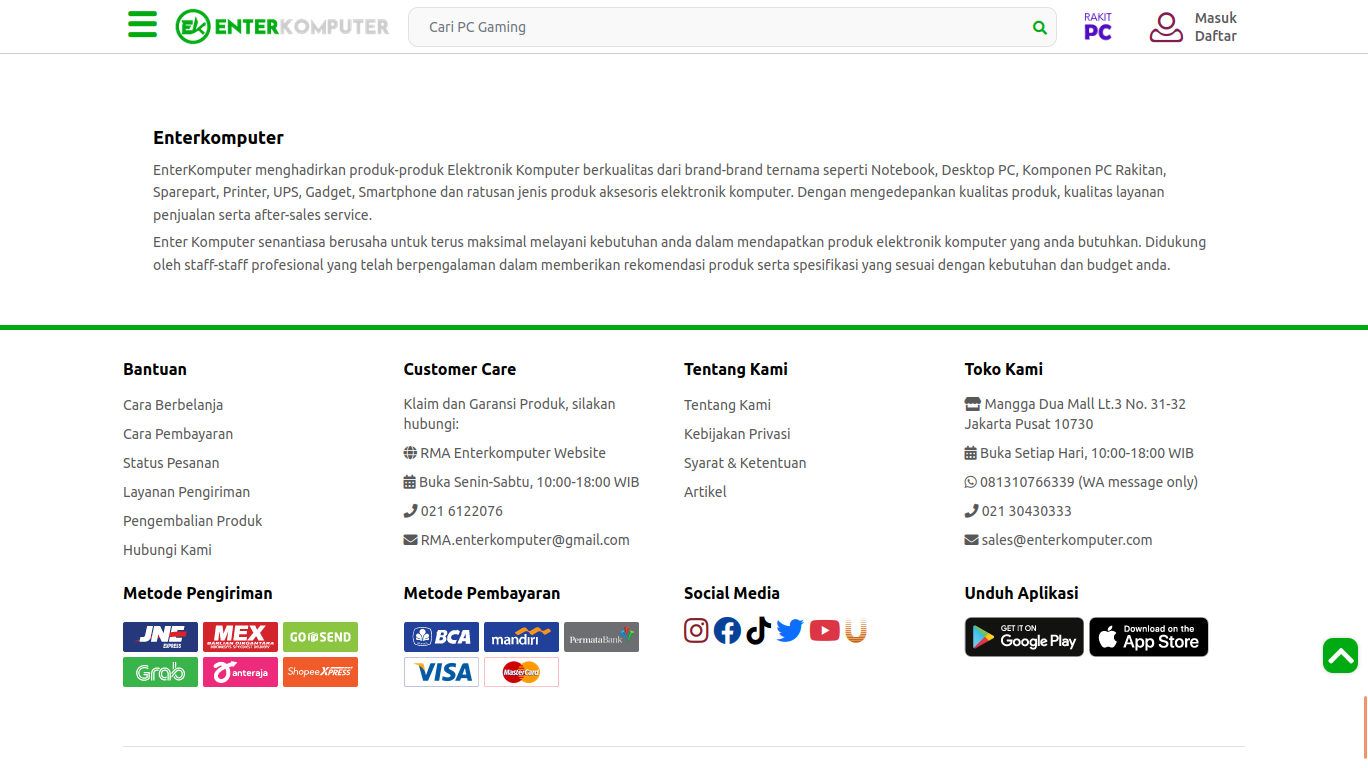
\includegraphics[width=\textwidth]{file-22.png}
\end{minipage}
\\
\begin{minipage}{0.30\textwidth}
    pada bagian ini pengguna dapat mencari barang dan menyaring nya
\end{minipage}
\hspace*{0.04\textwidth}
\begin{minipage}{0.65\textwidth}
    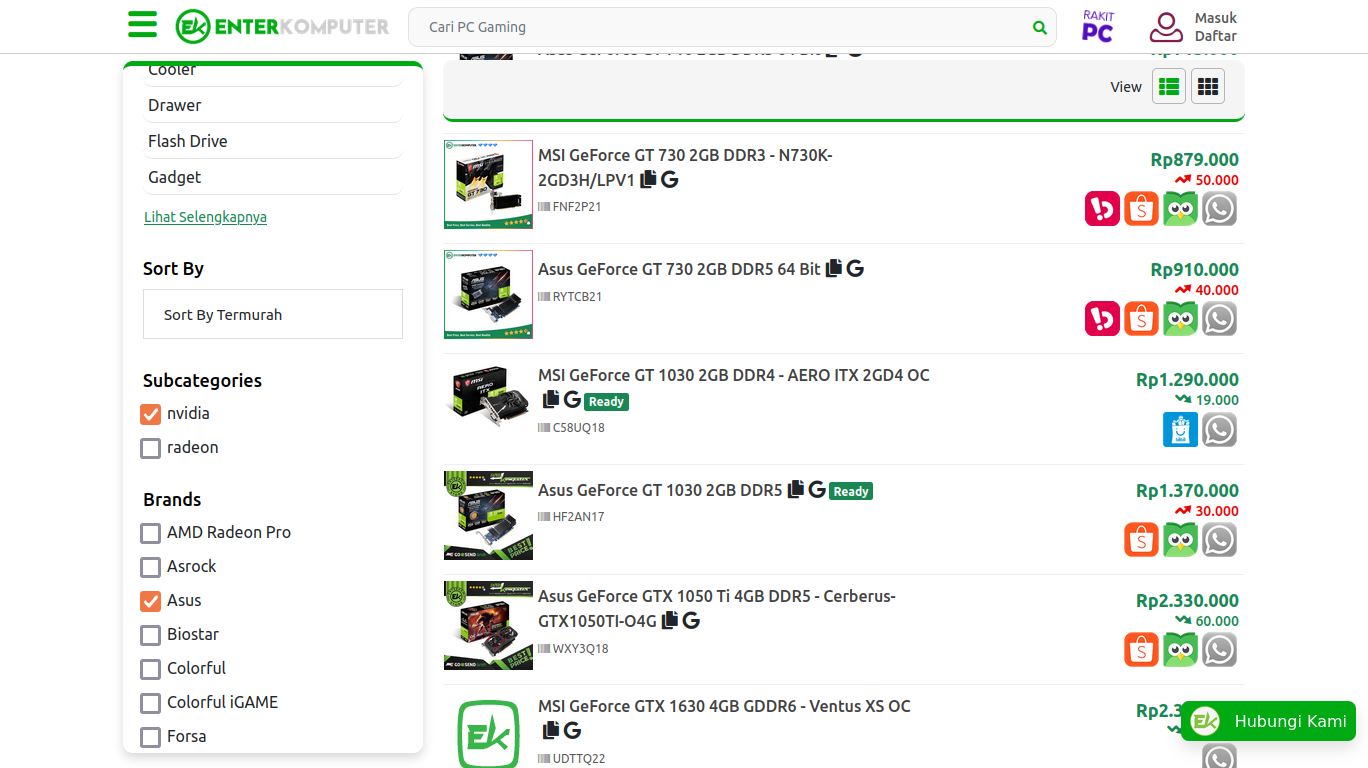
\includegraphics[width=\textwidth]{file-20.png}
\end{minipage}
\\
\begin{minipage}{0.30\textwidth}
    disini tersedia berbagai macam cara melakukan transaksi dan pengiriman, \textbf{financing} dan \textbf{pysical distribution}
\end{minipage}
\hspace*{0.04\textwidth}
\begin{minipage}{0.65\textwidth}
    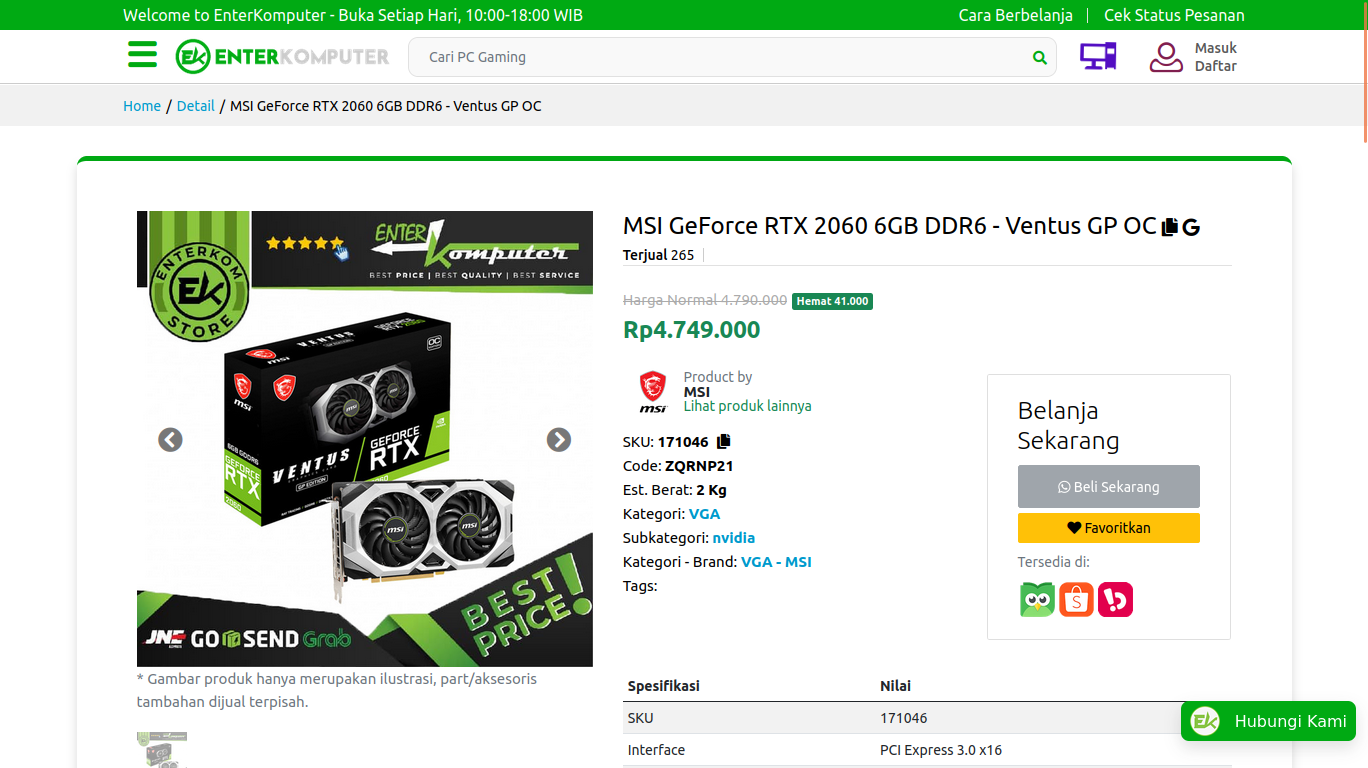
\includegraphics[width=\textwidth]{file-19.png}
\end{minipage}
\\
\begin{minipage}{0.30\textwidth}
    disini terdapat testimoni dan komentar, sebagai \textbf{fungsi promosi}
\end{minipage}
\hspace*{0.04\textwidth}
\begin{minipage}{0.65\textwidth}
    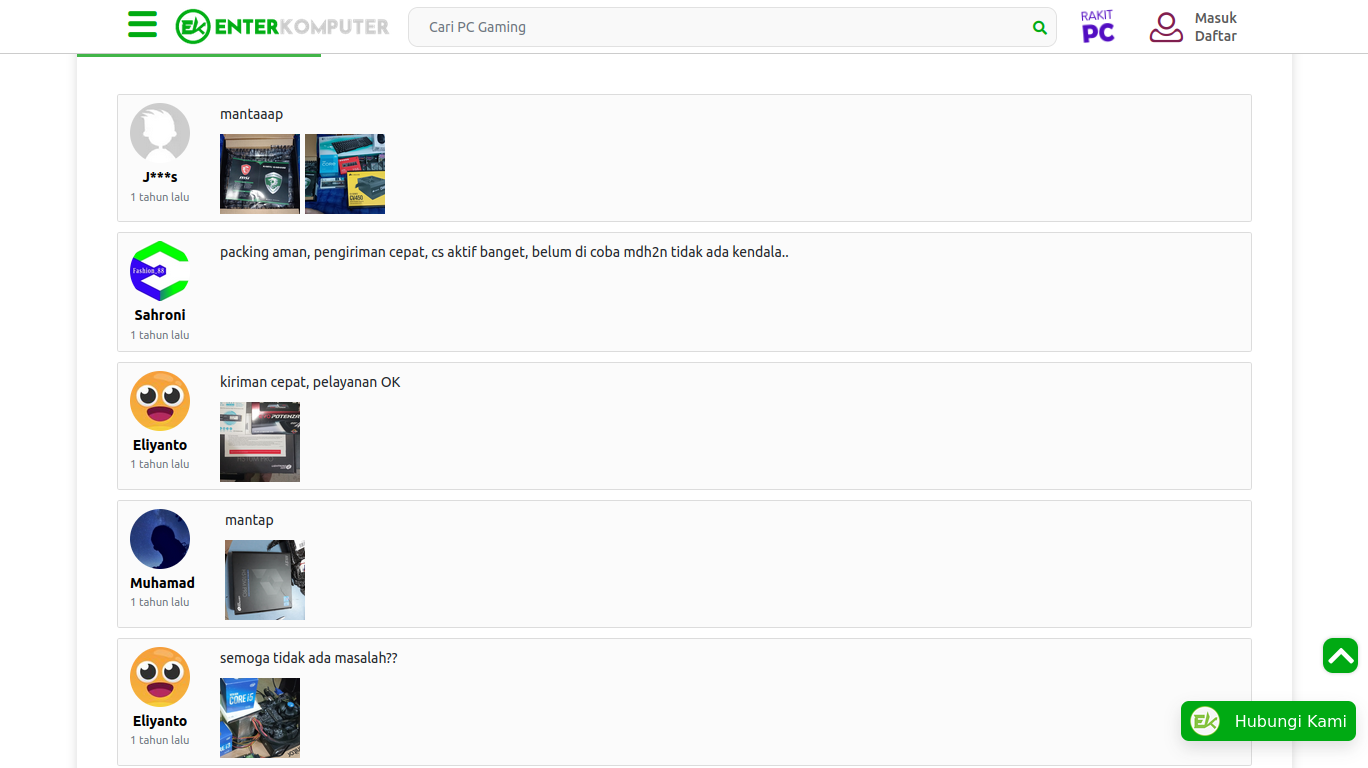
\includegraphics[width=\textwidth]{file-35.png}
\end{minipage}



\section*{Soal 3}
\noindent Kepuasan pelanggan dapat diukur dengan menggunakan indikator, \\
komentar komentar/ testimoni yang ditinggalkan pada halaman produk,\\
dengan pencatatan sistem yang tepat, menggunakan database dan web analytics, kita dapat mengetahui apabila seorang pengguna kembali lagi ataupun membeli lagi sebuah produk tertentu, atau dengan kata lain mengukur seberapa sering pengguna akan mencari dan menggunakan website untuk mencari kebutuhannya\\ 
kita juga dapat melihat kesuksesan website kita jika ditampilkan pada halaman depan google, juga search \emph{engine lainnya}, yang berarti website diakses oleh banyak orang dan SEO yang diterapkan sudah tepat.

\end{document}